\appendix

\section{Supplementary material}

\subsection{Retrieval and triplet accuracy}
\Cref{tab:scores-dialog} and \Cref{tab:scores-narration} show
the performance of several model configurations on the retrieval and
triplet tasks on the dialog and narration datasets respectively.
\todo{GC: Tables out of date}
 \begin{table}
   \centering
   \begin{tabular}{rlrr}
\toprule
 ID & Pretraining &  Recall@10 &  Triplet Acc \\
\midrule
 43 &          AV &      0.193 &        0.814 \\
 44 &           V &      0.084 &        0.728 \\
 45 &        None &      0.034 &        0.597 \\
\bottomrule
\end{tabular}

   \caption{Retrieval and triplet scores on dialog validation data.}
   \label{tab:scores-dialog}
 \end{table}

\begin{table}
   \centering
   \begin{tabular}{rlrr}
\toprule
 ID & Pretraining &  Recall@10 &  Triplet Acc \\
\midrule
 43 &          AV &      0.239 &        0.866 \\
 44 &           V &      0.166 &        0.822 \\
 45 &        None &      0.087 &        0.741 \\
\bottomrule
\end{tabular}

   \caption{Retrieval and triplet scores on narration validation data.}
   \label{tab:scores-narration}
 \end{table}

\subsection{Targeted Triplets Evaluation Sets}\label{app:targeted_triplets_eval}

To find commonly occurring nouns, adjectives, and verbs, we lemmatize and POS-tag all words in the transcripts of the validation dataset using spacy \citep{honnibal2020spacy}. Afterwards, we identify sets of all nouns $\{n_1, ..., n_n\}$, verbs $\{v_1, ..., v_o\}$ and adjectives $\{a_1, ..., a_p\}$ that occur at least 10 times in the validation data. Given these sets, we create sets of tuples $\{(n_1, n_2), (n_1, n_3), ..., (n_1, n_n), ...,  (n_{n-1}, n_n)\}$ for all combinations of nouns and verbs, respectively. For each of these tuples, we search the validation data for pairs of phrases $(p_k=[w_1, ..., w_x], p_l=[w_1, ..., w_y])$ with same length ($x=y$) and minimal difference regarding the tuple. That is, $n_1 \in p_1$, $n_2 \in p_2$, and if we replace $n_1$ with $n_2$ in $p_1$, it is equal to $p_2$. 

For example, if $n_1 = \text{"peppa"}$ and $n_2 = \text{"george"}$, the phrases $p_1 = [\text{"peppa", "loves", "jumping"}]$ and $p_2 = [\text{"george", "loves", "jumping"}]$ are phrases with minimal differences. A phrase can also be a single word.

We set the minimum phrase duration to 0.3 seconds (for shorter sequences, we do not expect that the video data contains enough semantic information for a model to distinguish between target and distractor). For each phrase $p_1$ we look for the \textit{longest} possible phrase $p_2$. \Cref{fig:num_samples_vs_duration} shows the distribution of samples per duration.

Based on each minimal pair, we construct two counter-balanced test triplets as described in the main text.

Figures \ref{fig:num_samples_NOUN_word}, and \ref{fig:num_samples_VERB_word} show the number of samples for each noun and verb for which at least 100 sets of test triplets were available (for no adjective there were enough samples found).


\begin{figure}
  \centering
  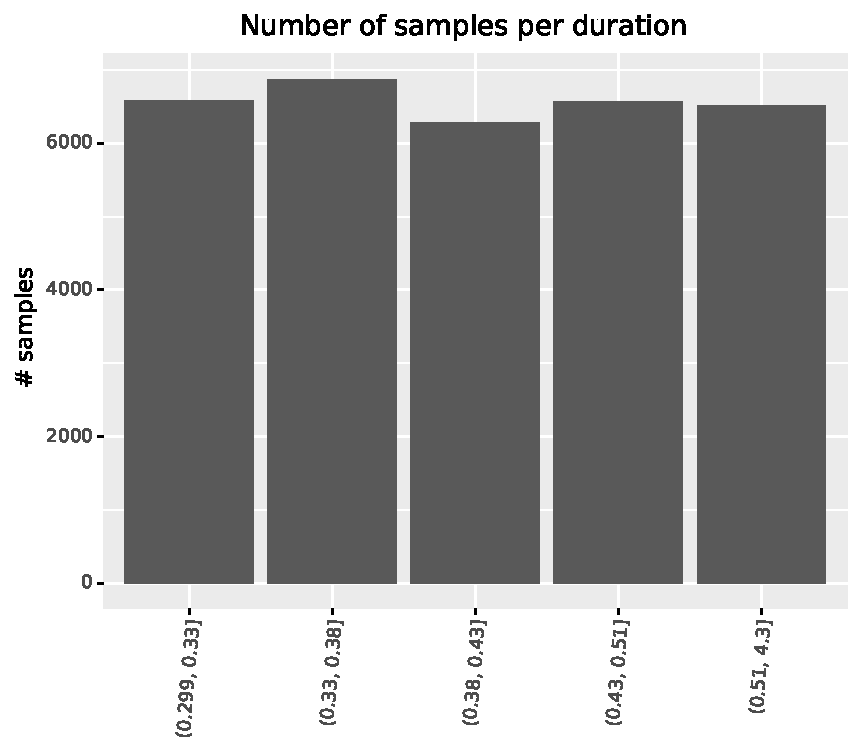
\includegraphics[width=\textwidth]{results/targeted_triplets/num_samples_per_duration.pdf}
  \caption{Number of samples per duration}
  \label{fig:num_samples_vs_duration}
\end{figure}


\begin{figure}
  \centering
  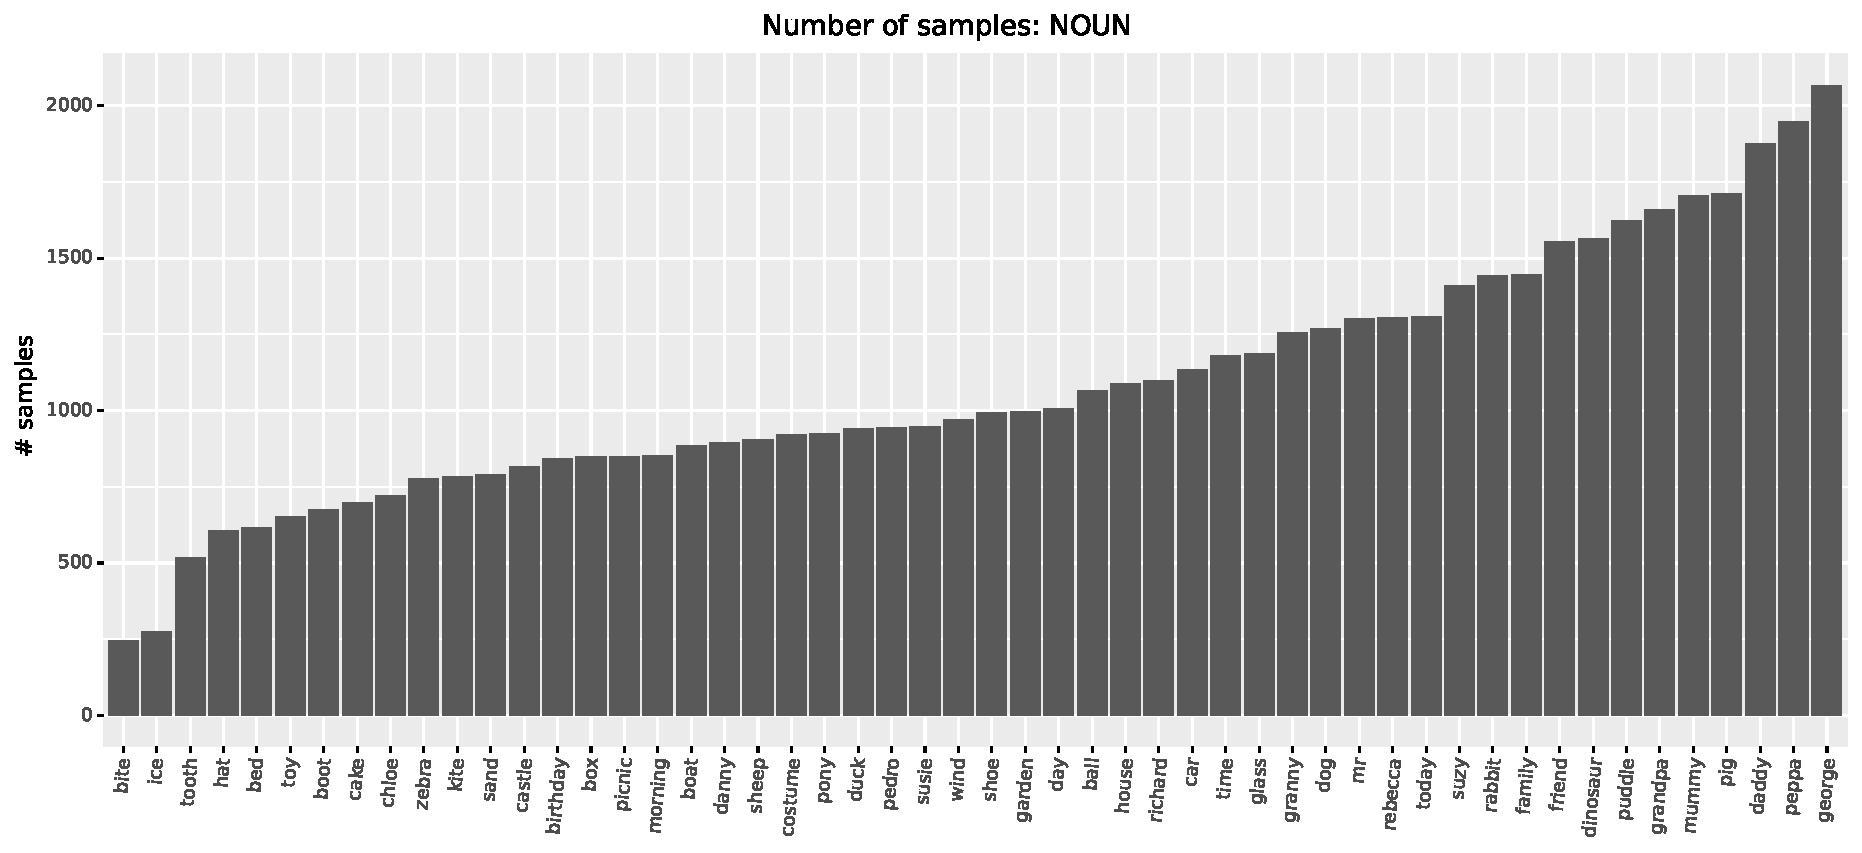
\includegraphics[width=\textwidth]{results/targeted_triplets/num_samples_per_word_NOUN.pdf}
  \caption{Number of samples: nouns}
  \label{fig:num_samples_NOUN_word}
\end{figure}

\begin{figure}
  \centering
  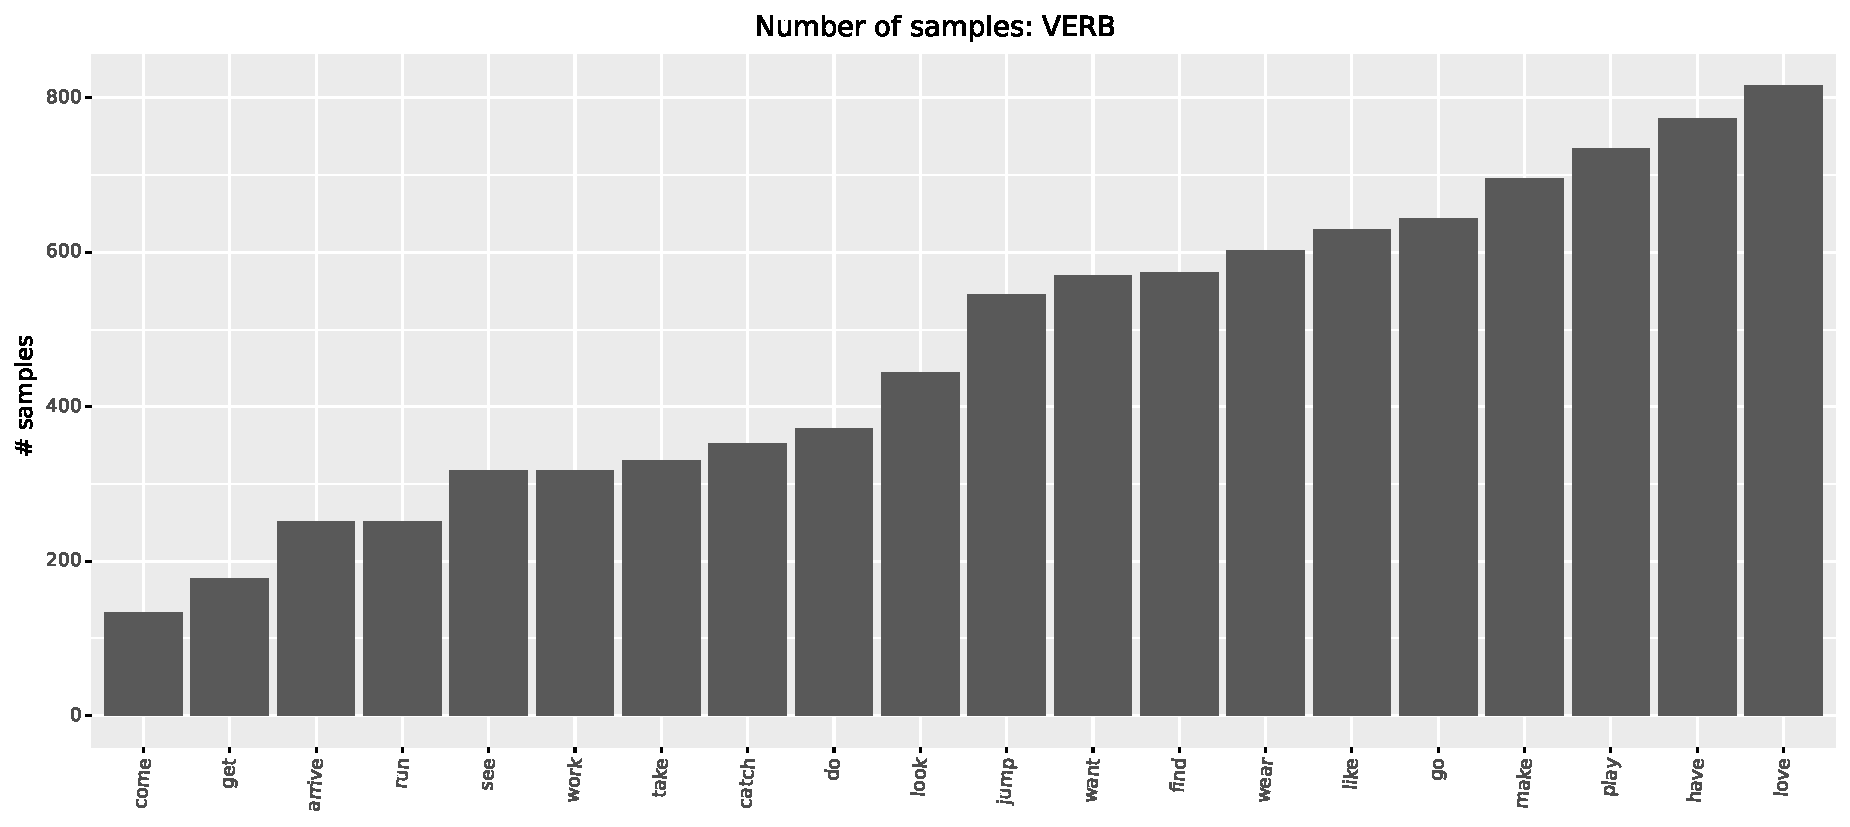
\includegraphics[width=\textwidth]{results/targeted_triplets/num_samples_per_word_VERB.pdf}
  \caption{Number of samples: verbs}
  \label{fig:num_samples_VERB_word}
\end{figure}

\subsection{Targeted Triplets Correlations}\label{app:targeted_triplets_correlations}

\Cref{fig:results_correlation_frequency_acc} shows the correlation between per-word accuracy and frequency of this word in the training data.
\Cref{fig:results_correlation_concreteness_acc} shows the correlation between per-word accuracy and concreteness scores.


\begin{figure}
  \centering
  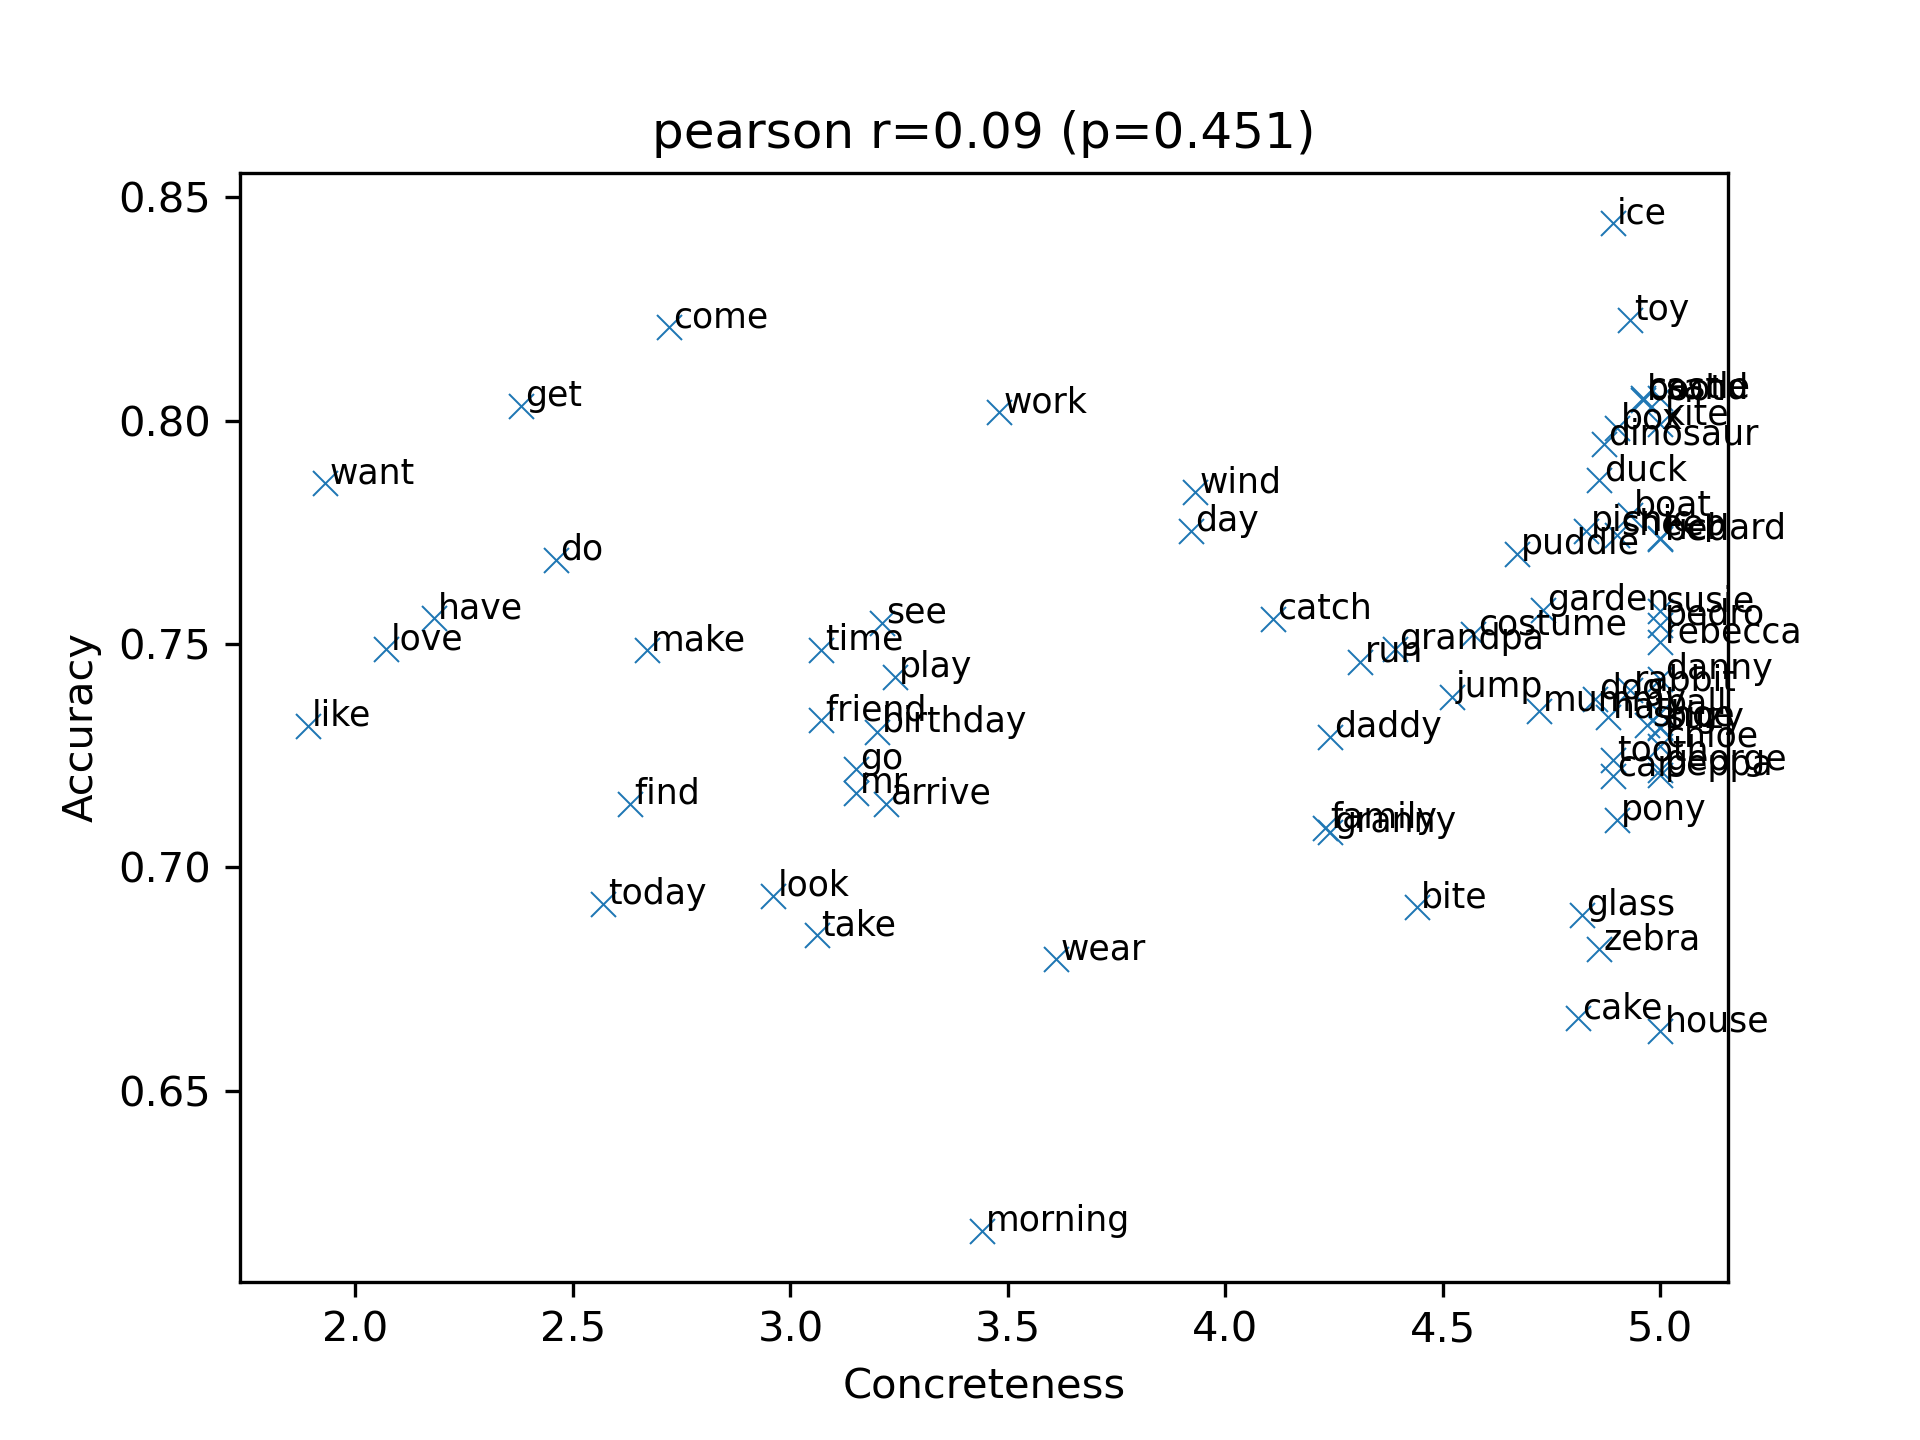
\includegraphics[width=\textwidth]{results/targeted_triplets/correlation_concreteness_acc_version_206980.png}
  \caption{Correlation between accuracy and log frequency.}
  \label{fig:results_correlation_frequency_acc}
\end{figure}

\begin{figure}
  \centering
  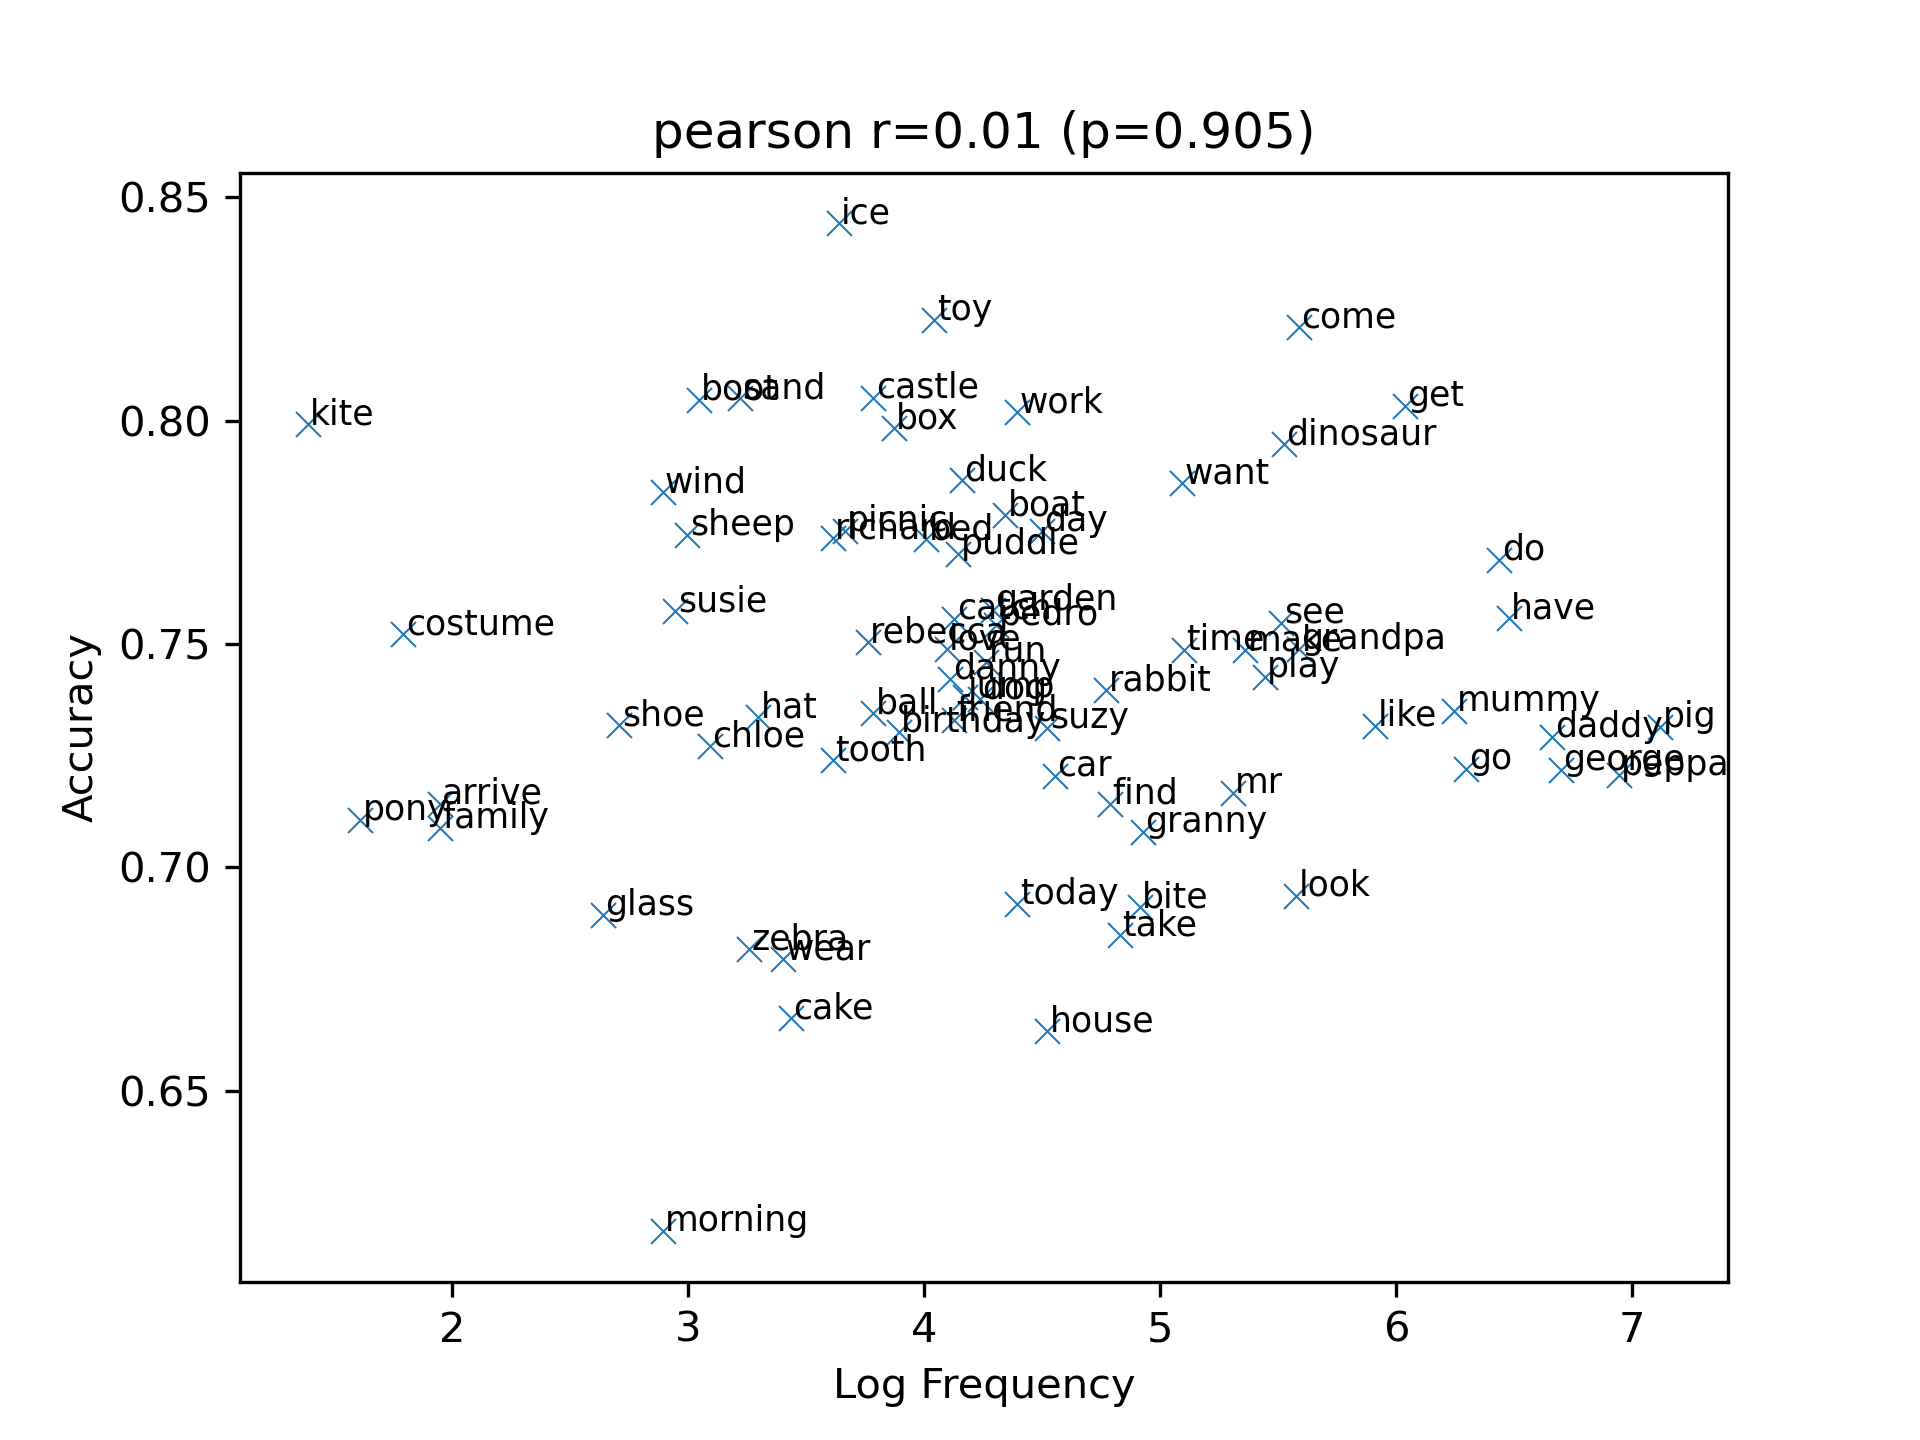
\includegraphics[width=\textwidth]{results/targeted_triplets/correlation_frequency_acc_version_206980.png}
  \caption{Correlation between accuracy and concreteness.}
  \label{fig:results_correlation_concreteness_acc}
\end{figure}

